\documentclass[11pt,twocolumn]{article}
\bibliographystyle{siam}

\usepackage[margin=0.75in]{geometry}
\usepackage{graphicx}

\title{\textbf{Team Zeta Project Report}\\
Linear Modeling and Time Series Analysis of Visual Pattern Recognition}
\author{
  Chen, Tzu-Chieh\\
  \texttt{tcchenbtx}
  \and
  Ho, Edith\\
  \texttt{edithhcw}
  \and
  Marediya, Zubair\\
  \texttt{zubair-marediya}
  \and
  Tran, Mike\\
  \texttt{miketranx4}
  \and
  Zhang, Dongping\\
  \texttt{dpzhang}
}

\begin{document}
\maketitle

\abstract{}
Visual recognition is a complicated process in our brain. 
Studying how the brain performs during it helps us improve our 
understanding of brain functionality. Therefore, we want to use the dataset 
from Haxby et al’s study, Distributed and Overlapping Representations of 
Faces and Objects in Ventral Temporal Cortex to answer the following questions.
If one presents different types of visual stimuli to a subject, would 
each stimulus evoke the same category-specific pattern of response in 
the ventral object vision pathway? Furthermore, can one fit a time series 
model to replicate the behavior of the BOLD signal from the responses? 
Also, can one use time series to match the correlation values of 
categories found in the study? \\

To study these questions, we performed linear modeling and ARIMA based 
times series analysis with this dataset. We found there is a consistent 
pattern for a subject to recognize one specific object. 
Even when we excluded maximally responding areas from the analysis, 
there was still a consistent pattern for visual recognition. Interestingly, 
our analysis showed that different subjects have different visual recognition 
patterns. Although these patterns differed greatly across subjects, 
they were consistent within subjects. In other words, even though subject
one has different patterns from subject two, they both had similar patterns 
among themselves when visually stimulated.\\

\section{Introduction}

In Haxby et al's study, \emph{Distributed and Overlapping Representations of 
Faces and Objects in Ventral Temporal Cortex}\cite{objectrec}, researchers
collected data from six subjects, including five females and one male. 
Different categories of pictures were presented to subjects as visual stimuli.
The categories are faces, cats, chairs, shoes, bottles, tools, houses, 
and a control category of phase-scrambled images.
The study aimed to answer the following questions: if we present 
different categories of visual stimuli to a subject, will category-specific 
response be evoked in the ventral cortex? \\

Each subject was placed into a functional magnetic resonance imaging 
(fMRI) facility for 12 experiment runs. One complete experiment run lasted 
300s. It began with 12s of rest, followed by 8 stimulus blocks of 24s duration, 
one for each category of visual stimuli. There were 12s intervals of 
rest between every two blocks, and the whole procedure ended 
with another 12s of rest. Each picture stimulus was presented
for 0.5s followed by an inter-stimulus interval of 1.5ms. 
12 stimuli were presented during each stimulus 
block, and a total of 96 stimuli in a complete experiment run.\\

In the study, the data collected for each subject were split into two 
runs: odd runs and even runs. Correlation was used as the indication of 
response similarity. Results from analyzing within-category and 
between-category correlations suggest that a lot of response patterns 
are overlapping. In the overlaps, there are parts of the cortex that respond 
more to a certain stimuli than others. The study defined these responses as 
maximal response. In order to gain more insights from the non-overlapping 
parts of the responses, the study tested whether the patterns of non-maximal 
responses carry category-related information. Voxels that responded maximally 
were excluded from this calculation of correlations. The results shown
that the removal of maximally responsive voxels from correlation calculations 
barely diminishes the accuracy of identification. The study concluded 
that both the pattern of large and small responses and the location 
of large responses carry category-related information and small responses
are an integral part of the representation.\\

\section{Data}

The study's curated dataset can be found and downloaded on the OpenfMRI 
database with ds105's accession number. The ds105 
sub-directory contains files detailing this study, including general 
information (README file), related research articles (references.txt), detail 
information and update for this released dataset (release\textunderscore 
history.txt), the MR repetition time (scan\textunderscore key.txt), the name 
(study\textunderscore key.txt), and the major task for this study 
(object viewing) (task\textunderscore key.txt). In addition, the models folder 
contains files with the key conditions (list of object categories) 
(condition\textunderscore key.txt) and the comparison setting in this study 
(tast\textunderscore contrasts.txt). \\

Subjects have individual directories storing their results. There are four 
sub-directories in each of the respective directories. The anatomy 
sub-directory contains high-resolution scans of the subject's head 
(highres001.nii.gz), mask for obtaining the ``brain only'' scans 
(highres001\textunderscore brain\textunderscore mask.nii.gz), and the 
``brain only'' anatomy result (highres001\textunderscore brain.nii.gz). 
The ``behav" sub-directory is empty since subject's behavior is irrelevant 
to this study. The ``model" sub-directory provides information such as the 
onset time (in seconds), and the duration and weighting for each conditions 
(object category) for the 12 task runs in this study. The ``BOLD" sub-directory 
contains fMRI results for all 12 task runs for each subject respectively. 
In each task run directory, we can find the fMRI result (bold.nii.gz) and 
a QA sub-directory with that run's time series analysis report, fMRI results
pre-processing and confound files, and visualization of the brain 
(nii files).\\ 


The preprocessed data for this ds105 dataset can be found and download from
https://nipy.bic.berkeley.edu/rcsds/. 
The processing applied to these fMRI scans includes: 
high-pass filtering in time (to remove low frequency drifts / noise, 
and registration to a standard anatomical template (the MNI template).\\

\section{Methods}

For each subject, there are eight condition files corresponding 
to each of the eight objects for each of the twelve runs. Each
condition file consists of time points of when the object was presented 
during the run. We started our analysis with subject 1, where we first wrote 
helper functions to identify and remove outliers.  Then we ran 
the event2neural function on subject 1's condition files, which returned an 
array of 121 zeros or ones. These values indicate
time intervals at which the subject was looking at the object.
We then used the numpy convolve function to convolve the BOLD signal 
onto the specified time intervals needed. After repeating this process 
for all objects, we created regressors and built our design matrix. 
Lastly, we fitted a linear model to the predicted BOLD signals 
from convolution, and gathered a mean RSS value. We then applied the contrast
function to investigate whether each object shows a response pattern in the 
brain.Unfortunately, initial images produced did not show sufficient contrast, 
making it difficult to observe patterns. Thus, we used smoothing techniques to 
produce better images. For smoothing, we applied Gaussian filters over an
array of voxel intensity values to generate images that are more appealing
to the human eye and easier to identify different parts of the brain.
The downside of this technique is that the new patterns identified can
potentially be false since the data is transformed. We then repeated our 
data analysis with the rest of the subjects. \\

We used various statistical methods and tests in our analysis. First,
we built a general linear model to provide estimates for the magnitude of
the response for respective stimulus. Then we applied this model to obtain
beta values for different objects. We then ran correlation analysis on the
beta values, which is further explained below. Moreover, the BOLD signal 
data are time series, and we performed appropriate analysis such as 
an object correlation table for each subject and an autoregressive integrated
moving average model to predict and fit the BOLD signal responses. 
Finally, in order to validate our models and data analysis, we looked 
at the mean squared errors to judge how well our model performs. \\

For correlation analysis, we divided all the runs into two groups (odd and 
even), and we aggregated all the results from each object within the group. 
Then, we computed the correlations between the average beta values of each 
object of each group and all objects in the opposite group. Take all the even 
runs where the subject was shown an image of a face as an example, we took 
the compiled array of beta values, and found the correlation between this 
array and that generated from all the odd runs where the subject was shown 
the images of a face, bottle, cat, chair, house, scissors, scrambledpix, and 
shoe respectively. This gives us 8 correlation values. By repeating the same 
procedures with all the other objects, we created a 8x8 correlation matrix. \\

\section{Results}

Since we started our analysis with subject 1, run001, we will first display 
those results. We performed initial analysis to attempt to identify specific 
brain region for recognizing specific object, such as face or house. 

Here are the outliers we identified and removed.
\begin{figure}[h!]
\centering
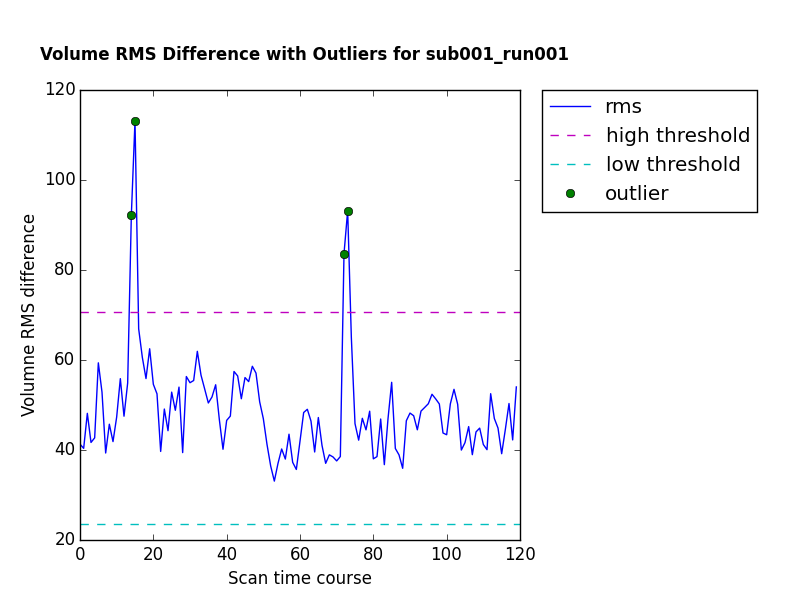
\includegraphics[width=90mm]{Volume_RMS_Difference_Outliers_sub001_run001.png}
\caption{Remove Outliers}
\end{figure}

Then, we generated task time course with the event2neural function.
\begin{figure}[h!]
\centering
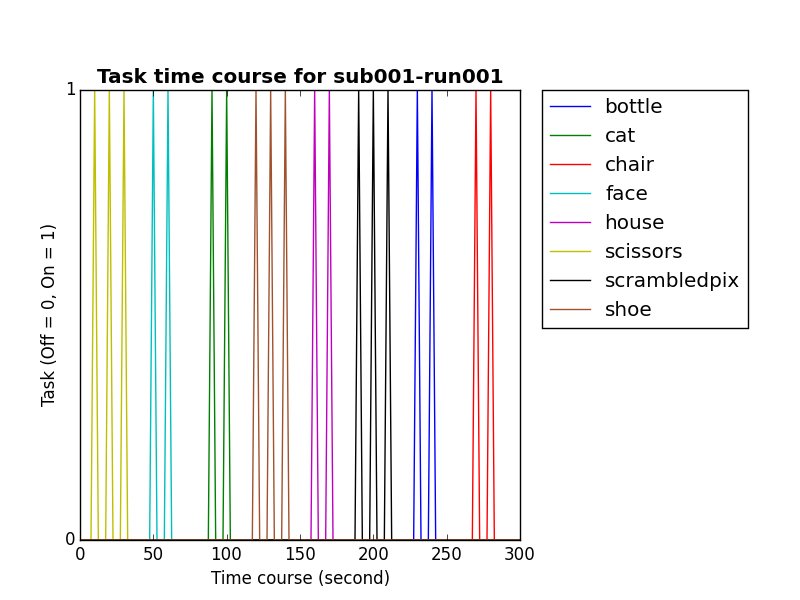
\includegraphics[width=90mm, height=60mm]{Task_time_course_sub001_run001.png}
\caption{Task Time Course}
\end{figure}

\pagebreak 

Afterwards, we performed convolution to generate predicted BOLD signals for 
this dataset.
\begin{figure}[h!]
\centering
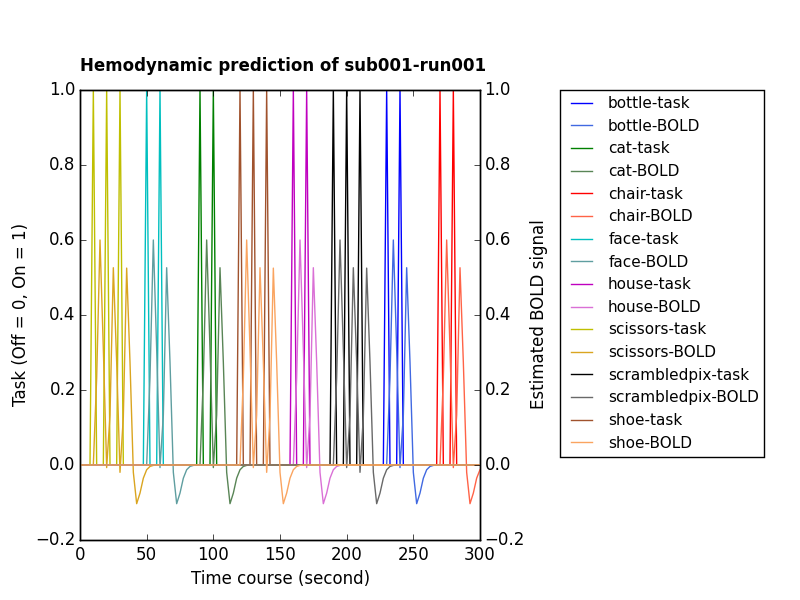
\includegraphics[width=90mm, height=60mm]{sub001_run001_bold_prediction.png}
\caption{Stimulation Bold}
\end{figure}

These convolved results for each objects were used as parameters in 
our design matrix for linear regression. To avoid the drifting problem, we also 
included two drift parameters in the design matrix (as shown i Fig. 4). 
The final design matrix was arranged as followed: 
bottle, cat, chair, face, house, scissors, scrambledpix, 
shoe, drift1, drift2, and ones (for background) 
\begin{figure}[h!]
\centering
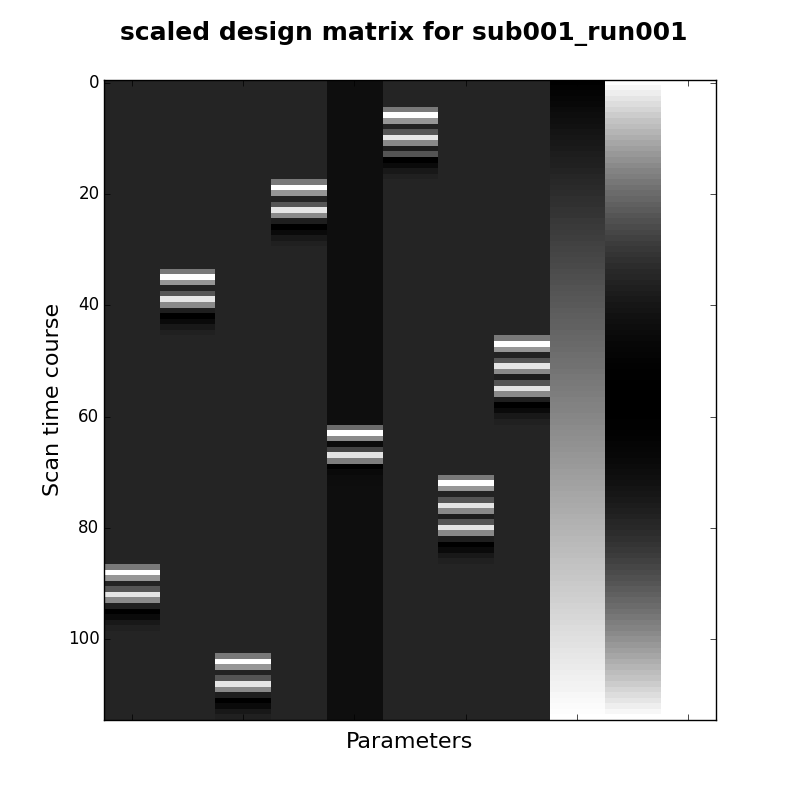
\includegraphics[width=90mm]{design_matrix_sub001_run001.png}
\caption{Design Matrix}
\end{figure}

As for the dataset, after removing the outliers and smoothing the data, 
we subset the brain region to perform analysis on brain areas.
We then used the design matrix to run linear modeling on the brain subset 
to get beta values. 
These beta bata values helped us to identify specific brain area and 
pattern for a subject under specific visual stimulation like house:

\begin{figure}[h!]
\centering
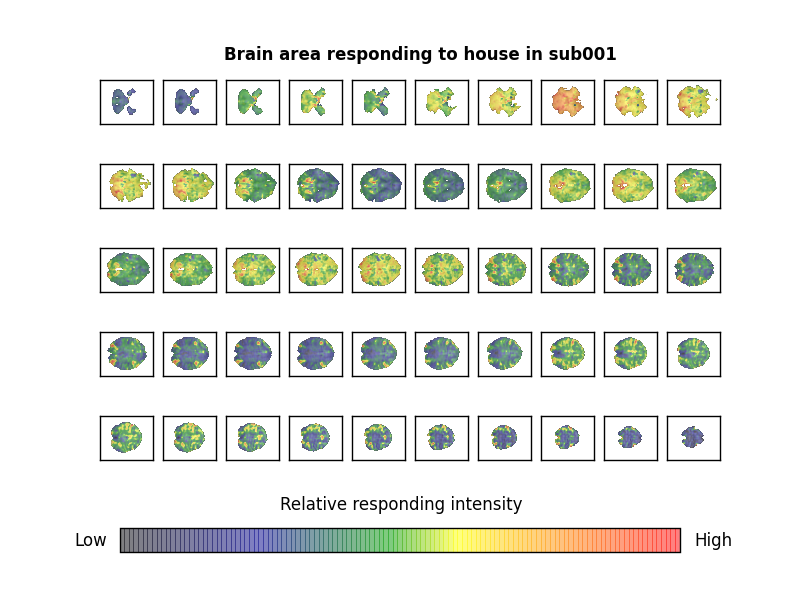
\includegraphics[width=90mm, height = 90mm]{betas_for_sub001_run001_house.png}
\caption{Betas for Sub001 Run001}
\end{figure}


As mentioned above, we want to run correlation analysis on the beta values.
We first focus on the correlation analysis on a 2D brain slice. To do that, 
we selected the most responding 2D brain area to perform the analysis. 
In the initial analysis, we tried to compare between run1 and 
run2 of subject1. We expected to see high correlation within category 
and low correlation between category. For instance, the run1 house and 
run2 house should have high correlation, whereas the run1 house and run2 face 
should have a low correlation. The 2D brain slice for the corresponding 
conditions are shown here:

\begin{figure}[h!]
\centering
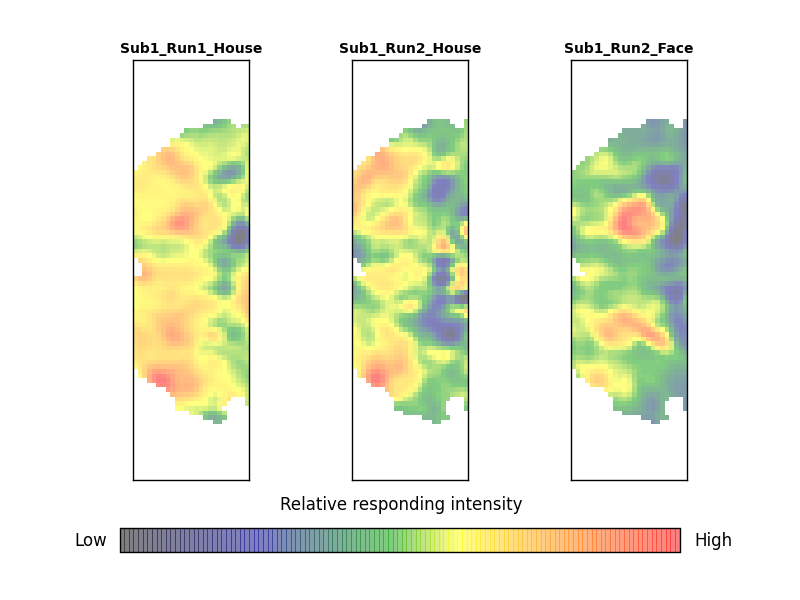
\includegraphics[width=90mm]{sub001_run_figure_compile.png}
\caption{Sub001 2D Compiled}
\end{figure}

Unfortunately, after performing this initial study, we didn’t get what 
we expected. However, some comparison across different runs shown our 
expected results. These observations indicated that there might be a 
variation in the results across runs. 
Therefore, to reduce the impact of variation across runs, we compiled the 
even run results and odd run results separately and used them to perform
correlation analysis. The mean results for even run and odd run shown similar
patter:

\begin{figure}[h!]                                                              
\centering                                                                      
\includegraphics[width=90mm]{odd_even_compile_sub001.png}                                                 
\caption{Sub001 Odd and Even run results}                                                    
\end{figure}

The within category correlation increased and is relatively  higher than
between category correlation (as shown in appendix). Excluding maximally
responding areas shown the similar pattern indicating the both the pattern of
large and small responses and the location of responses carry category-related
information.\\

Since the brain is a 3D structure, the visual recognition is processed in the
entire brain. Therefore, we next focus on the 3D brain slice to perform 
correlation analysis. The correlation table between even and odd runs are
listed below and shown as bar plots in appendix:

\begin{figure}[h!]                                                              
\centering                                                                      
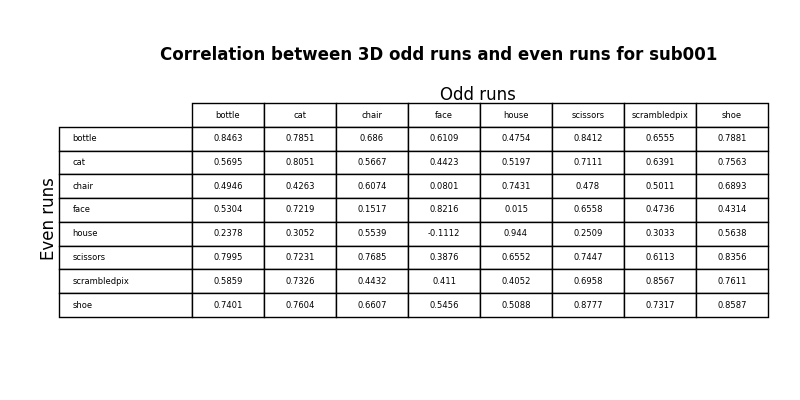
\includegraphics[width=90mm]{3d_correlation_table_sub001.png}                   
\caption{3D Correlation Table for Subject 1}                                    
\end{figure}                                                                    
                                                                                
\begin{figure}[h!]                                                              
\centering                                                                      
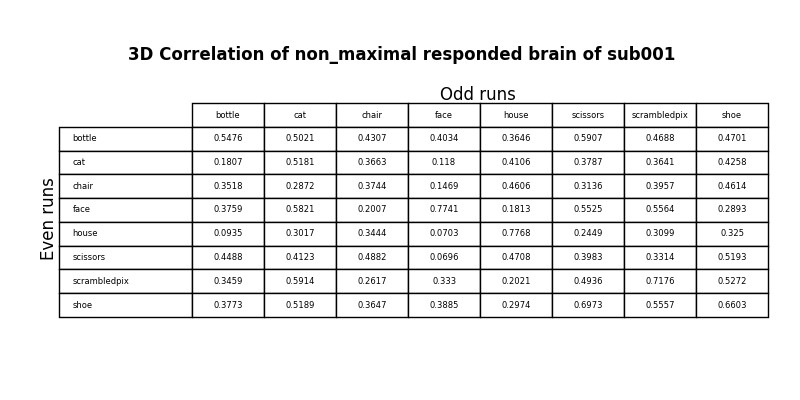
\includegraphics[width=90mm]{3d_non_max_correlation_table_sub001.png}           
\caption{3D Correlation Excluding Maximally Responding Voxels for Subject 1}    
\end{figure}     


As shown in the tables above, none of the correlation values are perfectly 1. 
The diagonal values are correlations between each object with their 
respective odd or 
even runs (within-category correlations). All within-category correlation 
values are larger than 0.6. For bottle, cat, face, house, scrambledpix, 
and shoe, the respective within-category correlations are higher than 
all of that object's between-category correlations with other objects.
For chair and scissors, the within-category correlations are not higher 
than all of their between-category correlations. Removing the maximally 
response area gave us the similar analytic results. This is consistent
with our findings on 2D correlation analysis.\\

Next, to further study whether the observation is consistent across subjects,
we performed the same analysis in all subjects of this dataset.
Interestingly, the brain pattern for visual recognition is different across
subjects. This might increase the variation for cross subjects analysis.
The mean correlation table was then created to statistically study the 
correlation pattern across subjects with and without maximally response areas:

\begin{figure}[h!]                                                              
\centering                                                                      
\includegraphics[width=90mm]{3d_total_correlation_table.png}                   
\caption{Mean 3D Correlation Table Across Subjects}
\end{figure}                                                                    
                                                                                
\begin{figure}[h!]                                                              
\centering                                                                      
\includegraphics[width=90mm]{3d_total_correlation_table_non_max.png}           
\caption{Mean 3D Correlation Table Excluding Maximally Responding Voxels Across
Subjects}    
\end{figure} 

Since there is high variation across subjects, all the correlation numbers
increased. However, the within category correlation was still relatively 
higher than between category correlation. The correlation without maximally
responded areas shown similar pattern. This again confirmed our and 
Haxby et al’s finding that both the pattern of   
large and small responses and the location of responses carry category-related  
information.\\


In time series correlation analysis, some questions we wanted to answer were
would the time series correlation tables be similar to ones produced from
the linear regression process if we looked at the raw nii data, how would
the correlations differ between the same and different objects, and was the
experiment designed in such a way so that correlations are the approximately
the same with different runs and subjects. The first step in the time series
analysis was retrieving a particular subset of the brain from the raw data.
This was done by getting the entire 4-D data, applying a mask on the 4-D data
to remove any noises, and using the same subsetted brain as the linear
regression process. Then, we averaged the subsetted brain into an array that
represents the BOLD signal responses from the beginning to the end of each run.
The array has a length of 121, which is the same as the length of each run.
Next, based on the condition files of each subject and run, we segmented the
array and created a time series array for each of the eight objects. The
condition files specified when an object was shown and for how long; thus,
giving us a particular range to subset precisely. Finally, we grouped the
object time series arrays into either even or odd runs. This allows us to
compare averaged even and odd object runs to one another and generate
Pearson Correlation coefficients. At the end of this analysis, six correlation
tables were generated.

\begin{figure}[h!]                                                              
\centering                                                                      
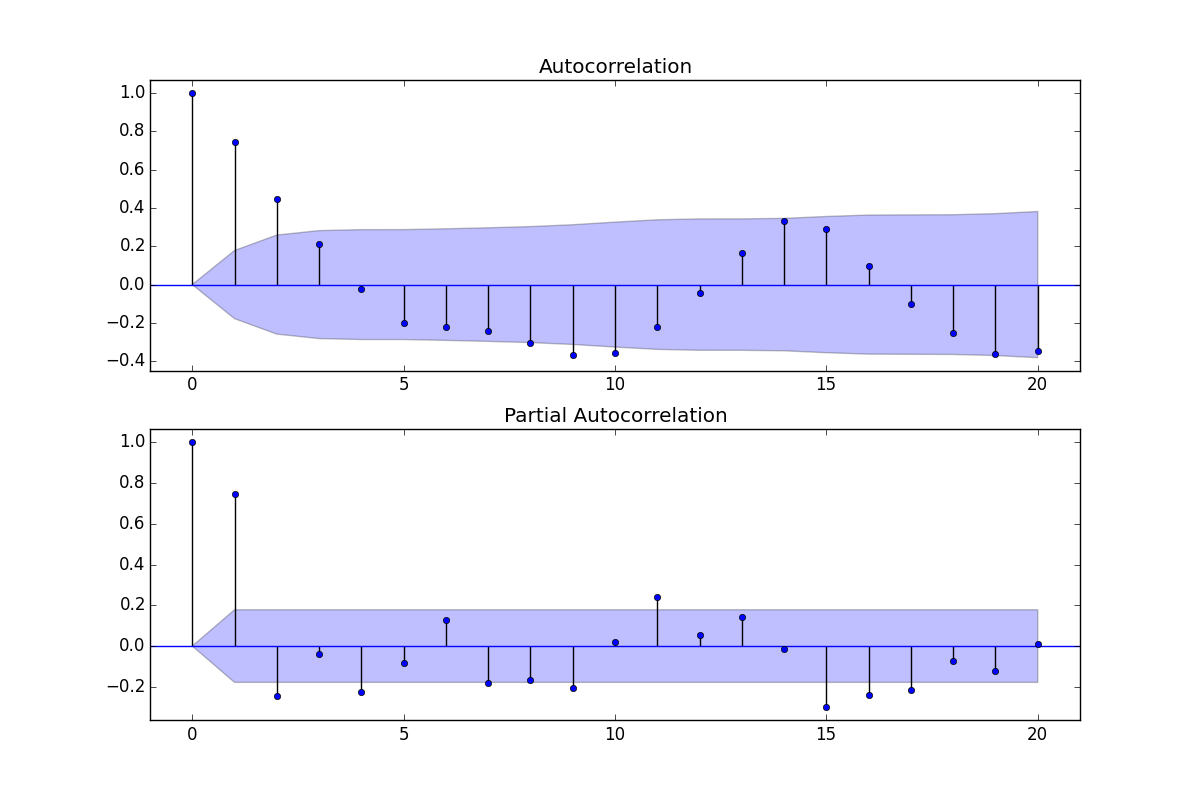
\includegraphics[width=90mm]{sub001_run001_corrFunc.png}                   
\caption{Autocorrelation and Partial Autocorrelation for Subject 1 Run 1}                                    
\end{figure}


On the time-side analysis, we were able to fit autoregressive integrated
moving average (ARIMA) models to the BOLD signal responses. This allowed us to
see how good of a fit a time series model is compared to the raw data and 
predict BOLD signal responses without having to know an object a subject is 
looking at. To see if we could initally fit a time-side model, we looked at
subject one run one's data. An autocorrelation and partial autocorrelation 
plot of the run's raw BOLD signals was generated. 

There is a significant lag cut-off after lag two in the 
partial autocorrelation plot, 
which means the autoregressive order should be at least two. The cut-off in 
the autocorrelation plot was at lag four, indiciating the moving average 
order should be four. To ensure these are the right orders for the ARIMA model, 
an auto.Arima() function was used to automate the parameter search process. 
In subject one run one, the best ARIMA model was ARIMA(2, 0, 0). 
Upon fitting the model, the residual's autocorrelation and partial 
autocorrelation plot were looked at to ensure a goodness of fit. 

\begin{figure}[h!]                                                              
\centering                                                                      
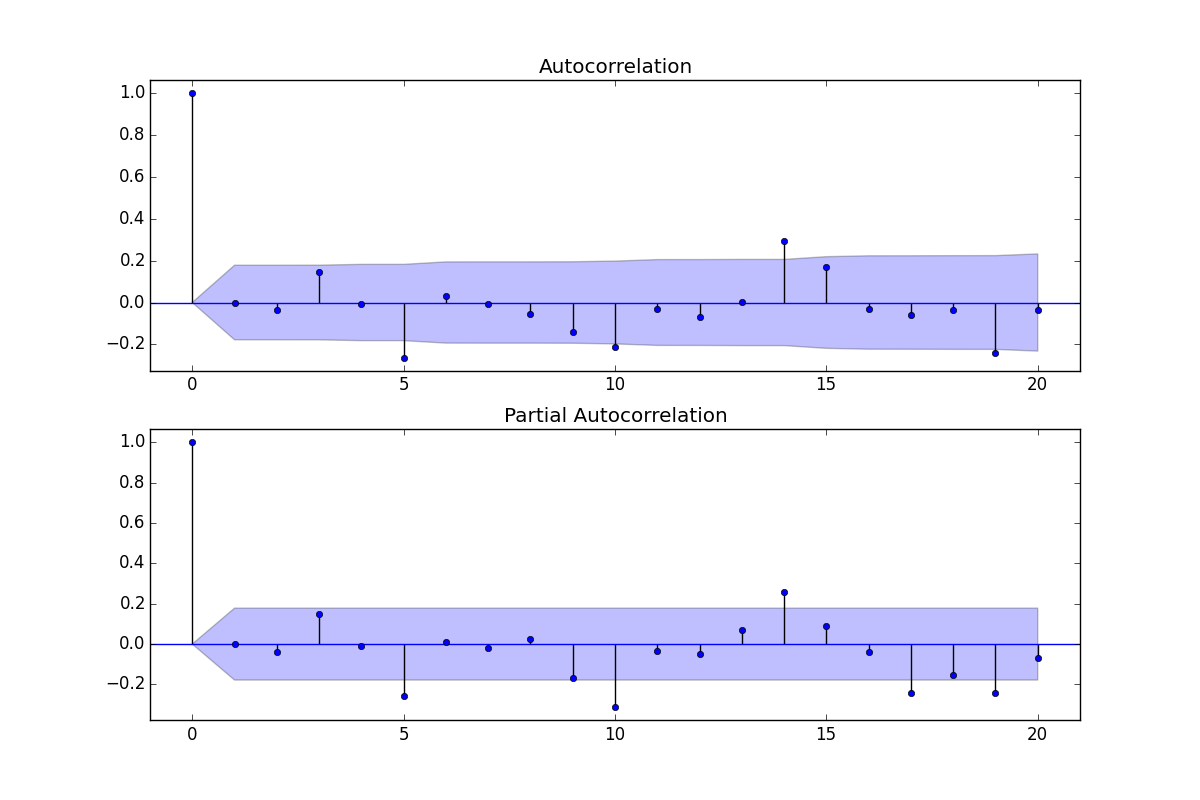
\includegraphics[width=90mm]{sub001_run001_residcorrFunc.png}                   
\caption{Autocorrelation and Partial Autocorrelation for Subject 1 Run 1 
Residuals}                                    
\end{figure}

In both plots, the significant lag cuts off after lag one;
thus, showing that the residuals have no serial correlation. In addition, the
Ljung-Box test was used to validate this assumption. It has a null hypothesis
that the residuals are independently distributed and uncorrelated, with an
altnerative hypothesis that they are correlated. The p-value came out to be
0.6071, so we accept the null. One trend that came up was that there were
no periods of volatility in the residuals plot; thus, we could not look into
an ARIMA-GARCH hybrid model.

\begin{figure}[h!]                                                              
\centering                                                                      
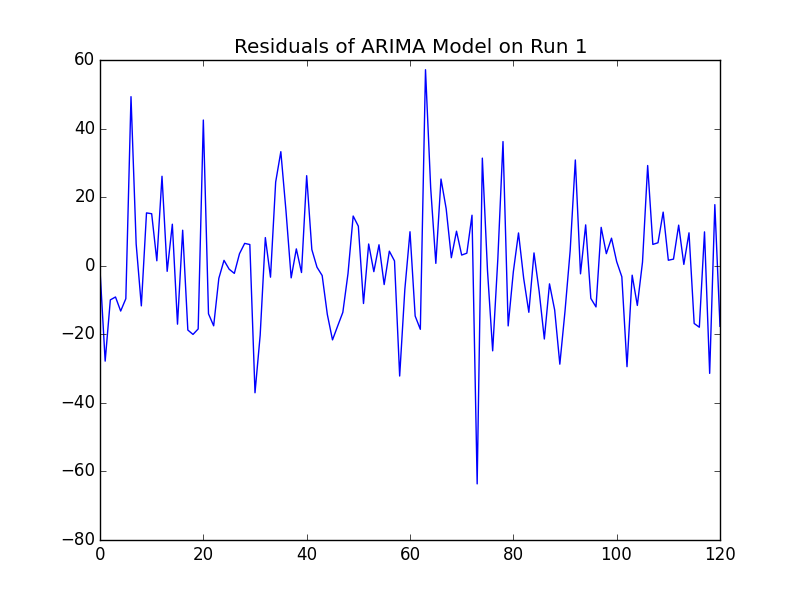
\includegraphics[width=90mm]{sub001_run001_residFit.png}                   
\caption{Residuals of ARIMA Model}                                    
\end{figure}

\begin{figure}[h!]                                                              
\centering                                                                      
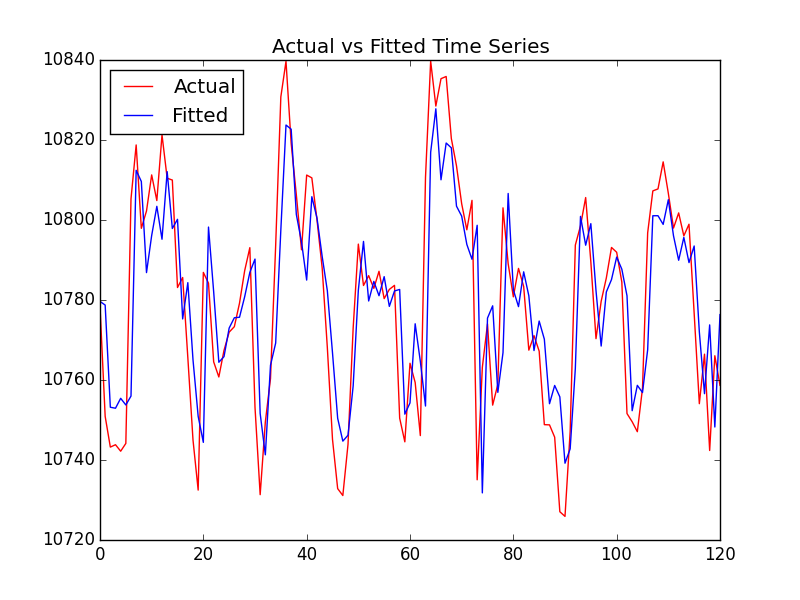
\includegraphics[width=90mm]{AFTS.png}                   
\caption{Actual vs Fitted Values of Subject 1 Run 1}                                    
\end{figure}


\section{Discussion}

Most of the within-category correlations we found are fairly similar than the 
paper?s. Some of the values from our analysis are higher than the paper?s, 
which could be 
due to the fact that we only analyzed correlations between runs for one 
subject, while the original research paper studied all subjects. It would make 
sense that correlations are higher when only analyzing brain activity from one 
brain. \\

Correlations between different objects (between-category correlations) seem 
fairly random, which also seem to be in line with the original paper?s finding. 
We observe that our between-category correlation values also tend to be higher 
than those from the paper. \\

To test the reproducibility of the study, we also redid our correlation 
analysis after excluding the maximally-responsive voxels. With the exception of 
some within-category correlations, most correlation values across all 
categories dropped after we removed the maximally-responsive voxels. This might 
be an indication that most of the highly correlated areas tend to have higher 
responses. \\

Looking at the correlation tables, the first thing that we noticed was that
the time series correlation tables were much more different from the linear
regression correlation tables. Even though the same subset of the brain was 
used, the time series tables exclusively had negative correlations, higher 
correlations with dissimilar objects against same objects, and even negative
correlations with the same objects. \\

\begin{figure}[h!]                                                              
\centering                                                                      
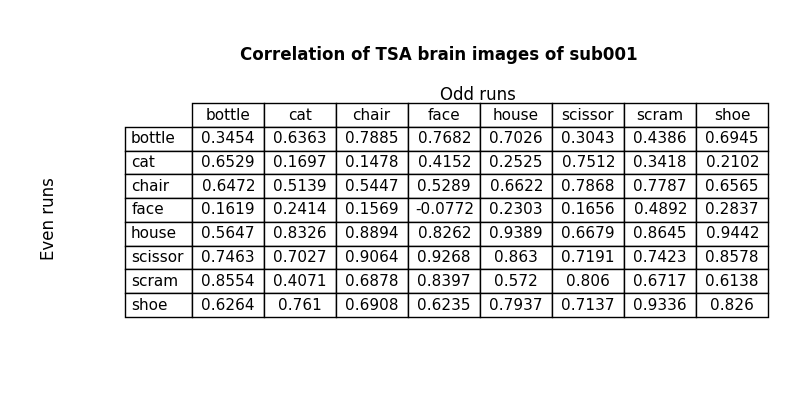
\includegraphics[width=90mm]{subtracted_correlation_table_sub001.png}                   
\caption{3D Correlation Time Series Table for Subject 1}                                    
\end{figure}

\begin{figure}[h!]                                                              
\centering                                                                      
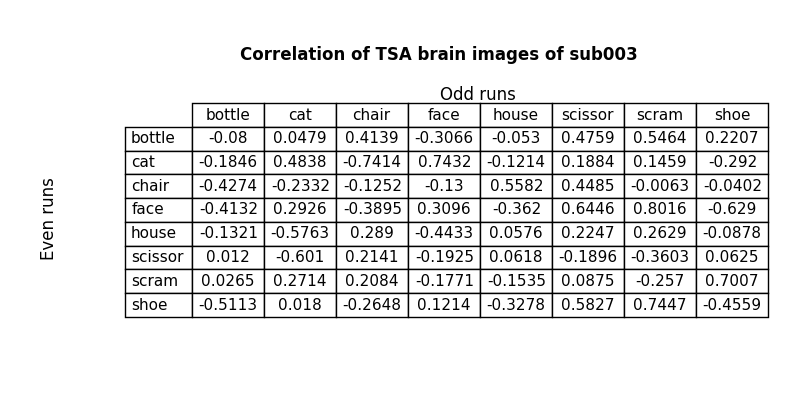
\includegraphics[width=90mm]{subtracted_correlation_table_sub003.png}                   
\caption{3D Correlation Time Series Table for Subject 3}                                    
\end{figure}


These differences could have come from how
the two processes were executed. For example, the linear regression process
involved convolving the data and transforming the data with beta values, 
whereas the time series analysis only looked at the raw data. Thus, this is
the most likely reason as to why the tables differed. The second thing the time
series correlation tables had was that across the six subjects, no two subjects
had similar correlation results. This confirms one of our hypothesis that 
the brain is a complex structure that will never give consistent results even
with a well designed experiment. What this means is that the BOLD signal
responses are not exactly 100\% comparable and it should be expected to have
contrasting correlation coefficients. One last point to bring up is that
the BOLD signals were not consistent across a subject's runs. In one run, a
cat BOLD signal would come out at an intensity of 10,800 and then in another,
it would come out to 10,500. One question we wanted to answer was given the
objects, can we predict the BOLD signal responses? Given that an object's
BOLD signal was never the same, this showed us that we couldn't answer that
particular question. Thus, we were unable to conclude anything regarding
predicting a BOLD signal given the objects. \\

In terms of time series analysis, now that there is a good model 
for one particular run, we can go about
answering the original questions we had with time-side analysis. When we 
plotted the actual to the fitted values, we see that the ARIMA model was 
able to capture the actual values very well. This allows us to get into
forecasting and predicting future responses. However, one limiation with
the python StatsModel package is that there are no forecasting methods
available. Thus, no further progress could be done unless R was available
as a tool. \\

There are a lot of problems that came up during our analysis. To begin with, 
since most of us have limited neuroscience knowledge, it was very difficult 
just to understand the study and the data itself. The research paper of the 
study uses specific and technical terms that make it hard to comprehend. 
More time was spent at the earlier stages rereading the 
original paper and exploring the data folders than expected, which slowed down 
our progress for analysis. Moreover, the values from correlation analysis 
did not come out as clean as we hoped, which also set our progress back. 
We did not end up have time to apply machine learning techniques for 
predictions as we originally splanned to. \\

\bibliography{project}

\newpage
\section{Appendix}
\begin{figure}[h!]
\centering
\includegraphics[width=90mm, height = 40mm]%
{sub001_2d_bottle_total_correlation_bar_both.png}
\caption{Sub001 2D Correlation: Bottle}
\end{figure}

\begin{figure}[h!]
\centering
\includegraphics[width=90mm, height = 40mm]%
{sub001_2d_cat_total_correlation_bar_both.png}
\caption{Sub001 2D Correlation: Cat}
\end{figure}

\begin{figure}[h!]
\centering
\includegraphics[width=90mm, height = 40mm]%
{sub001_2d_chair_total_correlation_bar_both.png}
\caption{Sub001 2D Correlation: Chair}
\end{figure}

\begin{figure}[h!]
\centering
\includegraphics[width=90mm, height = 40mm]%
{sub001_2d_face_total_correlation_bar_both.png}
\caption{Sub001 2D Correlation: Face}
\end{figure}


\begin{figure}[h!]
\centering
\includegraphics[width=90mm, height = 48mm]%
{sub001_2d_house_total_correlation_bar_both.png}
\caption{Sub001 2D Correlation: House}
\end{figure}

\begin{figure}[h!]
\centering
\includegraphics[width=90mm, height = 35mm]%
{sub001_2d_scissors_total_correlation_bar_both.png}
\caption{Sub001 2D Correlation: Scissor}
\end{figure}

\begin{figure}[h!]
\centering
\includegraphics[width=90mm, height = 34mm]%
{sub001_2d_scrambledpix_total_correlation_bar_both.png}
\caption{Sub001 2D Correlation: Scram}
\end{figure}

\begin{figure}[h!]
\centering
\includegraphics[width=90mm, height = 34mm]%
{sub001_2d_shoe_total_correlation_bar_both.png}
\caption{Sub001 2D Correlation: Shoe}
\end{figure}


\newpage


\begin{figure}[h!]
\centering
\includegraphics[width=90mm]%
{sub001_3d_bottle_total_correlation_bar_both.png}
\caption{Sub001 3D Correlation: Bottle}
\end{figure}

\begin{figure}[h!]
\centering
\includegraphics[width=90mm]%
{sub001_3d_cat_total_correlation_bar_both.png}
\caption{Sub001 3D Correlation: Cat}
\end{figure}

\begin{figure}[h!]
\centering
\includegraphics[width=90mm]%
{sub001_3d_chair_total_correlation_bar_both.png}
\caption{Sub001 3D Correlation: Chair}
\end{figure}

\begin{figure}[h!]
\centering
\includegraphics[width=90mm]%
{sub001_3d_face_total_correlation_bar_both.png}
\caption{Sub001 3D Correlation: Face}
\end{figure}

\begin{figure}[h!]
\centering
\includegraphics[width=90mm]%
{sub001_3d_house_total_correlation_bar_both.png}
\caption{Sub001 3D Correlation: House}
\end{figure}

\begin{figure}[h!]
\centering
\includegraphics[width=90mm]%
{sub001_3d_scissors_total_correlation_bar_both.png}
\caption{Sub001 3D Correlation: Scissor}
\end{figure}

\begin{figure}[h!]
\centering
\includegraphics[width=90mm]%
{sub001_3d_scrambledpix_total_correlation_bar_both.png}
\caption{Sub001 3D Correlation: Scram}
\end{figure}

\begin{figure}[h!]
\centering
\includegraphics[width=90mm]%
{sub001_3d_shoe_total_correlation_bar_both.png}
\caption{Sub001 3D Correlation: Shoe}
\end{figure}

\newpage

\begin{figure}[!h]
\centering
\includegraphics[width=90mm, height = 43mm]%
{2d_total_correlation_bar_both_bottle.png}
\caption{Cross Subject 2D Correlation: Bottle}
\end{figure}

\begin{figure}[h!]
\centering
\includegraphics[width=90mm, height = 44mm]%
{2d_total_correlation_bar_both_cat.png}
\caption{Cross Subject 2D Correlation: Cat}
\end{figure}

\begin{figure}[h!]
\centering
\includegraphics[width=90mm, height = 43mm]%
{2d_total_correlation_bar_both_chair.png}
\caption{Cross Subject 2D Correlation: Chair}
\end{figure}

\begin{figure}[h!]
\centering
\includegraphics[width=90mm, height = 44mm]%
{2d_total_correlation_bar_both_face.png}
\caption{Cross Subject 2D Correlation: Face}
\end{figure}

\begin{figure}[h!]
\centering
\includegraphics[width=90mm]%
{2d_total_correlation_bar_both_house.png}
\caption{Cross Subject 2D Correlation: House}
\end{figure}

\begin{figure}[h!]
\centering
\includegraphics[width=90mm]%
{2d_total_correlation_bar_both_scrambledpix.png}
\caption{Cross Subject 2D Correlation: Scram}
\end{figure}

\begin{figure}[h!]
\centering
\includegraphics[width=90mm]%
{2d_total_correlation_bar_both_shoe.png}
\caption{Cross Subject 2D Correlation: Shoe}
\end{figure}

\begin{figure}[h!]
\centering
\includegraphics[width=90mm]%
{2d_total_correlation_bar_both_scissors.png}
\caption{Cross Subject 2D Correlation: Scissors}
\end{figure}

\newpage

\begin{figure}[h!]
\centering
\includegraphics[width=90mm]%
{3d_total_correlation_bar_both_bottle.png}
\caption{Cross Subject 3D Correlation: Bottle}
\end{figure}

\begin{figure}[h!]
\centering
\includegraphics[width=90mm]%
{3d_total_correlation_bar_both_cat.png}
\caption{Cross Subject 3D Correlation: Cat}
\end{figure}

\begin{figure}[h!]
\centering
\includegraphics[width=90mm]%
{3d_total_correlation_bar_both_chair.png}
\caption{Cross Subject 3D Correlation: Cat}
\end{figure}

\begin{figure}[h!]
\centering
\includegraphics[width=90mm]%
{3d_total_correlation_bar_both_face.png}
\caption{Cross Subject 3D Correlation: face}
\end{figure}

\begin{figure}[h!]
\centering
\includegraphics[width=90mm]%
{3d_total_correlation_bar_both_house.png}
\caption{Cross Subject 3D Correlation: House}
\end{figure}

\begin{figure}[h!]
\centering
\includegraphics[width=90mm]%
{3d_total_correlation_bar_both_scrambledpix.png}
\caption{Cross Subject 3D Correlation: Scram}
\end{figure}

\begin{figure}[h!]
\centering
\includegraphics[width=90mm]%
{3d_total_correlation_bar_both_shoe.png}
\caption{Cross Subject 3D Correlation: shoe}
\end{figure}

\begin{figure}[h!]
\centering
\includegraphics[width=90mm]%
{3d_total_correlation_bar_both_scissors.png}
\caption{Cross Subject 3D Correlation: Scissors}
\end{figure}

\end{document}
